\documentclass[11pt,dvipsnames]{scrreprt}%oldschool: report

\usepackage[utf8]{inputenc}
\usepackage{ngerman}
\usepackage{fullpage} % kleinere Ränder

\usepackage{comment} % für größere comments: \begin{comment} ... \end{comment}

% *** für eingefügte (pdf-)Grafiken
\usepackage[pdftex]{graphicx} 
%\pdfminorversion=6
% ***

\usepackage{float}
\restylefloat{figure}

\usepackage{enumerate} %für geschachtelte Aufzählungen


\linespread{1.25}
\usepackage{amsmath} %Matheformeln usw.
\usepackage{amssymb} %mathfrak

\usepackage[bookmarks=true]{hyperref} % hyperrefs aktivieren
\setcounter{secnumdepth}{3} %Numerierung bis Tiefe 3, also ab \paragraph ohne

% *** java listings
\usepackage{xcolor,luximono,listings}
\usepackage{listings}
\lstloadlanguages{PYTHON,SQL,XML,JAVA}
\usepackage{courier} % courier schrift
\lstset{
	language=Java, 
	basicstyle=\ttfamily, 
	tabsize=4,
	literate= {Ö}{{\"O}}1 {Ä}{{\"A}}1 {Ü}{{\"U}}1 {ß}{{\ss}}2 {ü}{{\"u}}1
 	{ä}{{\"a}}1 {ö}{{\"o}}1
}
% end listing ***

% *** requirements commands definition
% use \initReqgrp{<group-ref>} to set group
% use \req{<title>}{<requirement-ref>} to set a main requirement (label inclusive)
% use \subreq{<title>}{<subrequirement-ref> to set a sub requirement (label inclusive)

\gdef \reqGrp{x}% 										requirement group prefix
\gdef \reqMain{x}% 										requirement reference shortcut
\gdef \reqSub{x}% 										requirement reference shortcut
\newcounter{cntReqGrp}% 								requirement group counter
\newcounter{cntReq}[cntReqGrp]% 						main requirement counter
\newcounter{cntSubReq}[cntReq]% 						sub requirement counter
\newcommand{\reqPrefix}{/}
\newcommand{\reqPostfix}{/}
\renewcommand{\thecntReq}{\reqPrefix\reqGrp-\arabic{cntReq}\reqPostfix}% 		set output or cntReq
\renewcommand{\thecntSubReq}{\reqPrefix\reqGrp-\arabic{cntReq}.\arabic{cntSubReq}\reqPostfix}% set output of cntSubReq
\newcommand{\req}[2] {% 								define new requirement, input: title, reference shortcut
	\refstepcounter{cntReq}% 								update counter
	\gdef \reqMain{#2}% 								update requirement reference
	\thecntReq\  #1% 									set output \end{reqtxt} label text
	\label{req:\reqGrp:#2}% 							set label 
}

\newcommand{\subreq}[2] {% 								define new sub requirement, input: title, reference shortcut
	\refstepcounter{cntSubReq}% 							update counter
	\gdef \reqSub{#2}% 									update requirement reference
	\thecntSubReq\  #1% 			set output text 
	\label{req:\reqGrp:\reqMain:\reqSub}% 				set label
}

\newcommand{\initReqgrp}[1] {% 							init new requirement group, input: prefix
	\gdef \reqGrp{#1}% 									overwrite variable reqgrp
	\refstepcounter{cntReqGrp}% 						update group counter
}
% *** end requirements commands


% *** shortcuts
\def \arc{ARC}
\def \ci{Christoph Piechula}
\def \cii{Christoph Cwelich}
\def \ciii{Christopher Pahl}
\def \eddy{Eduard Schneider}
\def \flo{Florian Bauer}
\def \sab{Sabrina Biersack}

% ***

%*** title etc.
\title{Dokumentation\\
Praktikum Software Entwicklung }
\author{Dozent: Prof. Dr. Richard Göbel \\
Beteiligte Studenten: \\
\sab, \\ \flo, \\ \eddy, \\ \ci, \\ \cii, \\ \ciii
}
\date{\today}
%***

%newcommands
%\newcommand{\neuesKommando}{Was zu tun ist}
\newcommand{\todo}[1]{\Huge{TODO: #1}}
\newcommand{\code}[1]{\lstinline{#1}}
\newcommand{\liable}[1]{Verantwortlich: #1 \\}
\begin{document}

\maketitle

\tableofcontents

\part{Spezifikation}
\chapter{Übersicht}
Über einen konfigurierbaren Crawler können Inhalte von Webseiten bis zu einer bestimmten Tiefe
aus dem Internet in ein Archiv geladen werden. Da dies parallelisiert erfolgen soll,
müssen die Daten nach dem Herunterladen von temporären Verzeichnissen in das gemeinsame
Archivverzeichnis synchronisiert werden. Der aus der URL extrahierte Pfad der Dateien wird
dabei auf das Archiv abgebildet, wobei jede Datei in einen eigenen Archivordner verschoben wird.\\

Beim Crawlvorgang werden zusätzlich Metadaten der heruntergeladenen Dateien erstellt. 
Diese werden in einer Datenbank und als XML-Datei im jeweiligen Archivordner gespeichert.
Die Datenbank soll dabei wieder aus den XML-Daten rekonstruierbar sein. \\ 

Außerdem sollen Filter eingehängt werden können, die bereits in den TMP-Ordnern ungültige Dateien löschen.
Über eine Java-Schnittstelle kann anschließend wieder auf die Daten zugegriffen werden.
Hierzu müssen sich Clients über eine vorgegebene Schnittstelle beim Textarchiv anmelden.
Die Clients werden anschließend bei Änderungen oder neuen Einträgen benachrichtigt und können sich selbstständig über die Schnittstelle einen beliebigen Stand der Daten herunterladen und an Analysetools weitergeben.
Dabei sollen auch neue Dateien den Archivordnern hinzugefügt werden können.
Ebenso sollen die oben genannten XML-Daten um neue Nodes erweiterbar sein.
Zu Vorführzwecken wird ein Testanalysetool erstellt.


 

\chapter{Datenmodell der Metadaten} \label{spec:model}
An dieser Stelle wird bereits ein vereinfachtes Datenmodell festgelegt, 
welches später auf Datenbank und XML-Daten umgesetzt wird und zentrale Metadaten 
der heruntergeladenen Dateien erfassen soll. 

Für jede Datei wird dabei ein solcher Satz von Metadaten angelegt.
Die Metadaten sollen vor allen Dingen Such- und Sortieraufgaben erleichtern. 

\begin{table}[h]
\centering
\begin{tabular}{|l|l|l|}	
	\hline
	Name 		& Datentyp 				& Beschreibung \\
	\hline
	url 		& String 				& Original URL der Datei\\
	\hline
	mimeType	& String 				& MIME-Typ der Datei\\
	\hline
	title 		& String 				& Soweit vorhanden, wird der Titel der Seite \\ 
	 			& 						& gespeichert \\ 
	\hline
	path 		& String 				& Dateipfad zum Archivordner der Datei im Webarchiv \\
	\hline
	domain 		& String 				& Name der Domain \\
	\hline
	crawlTime 	& Timestamp 			& Beginn des Crawls \\
	\hline
	createTime 	& Timestamp 			& Erzeugungszeitpunkt der Datei \\
	\hline
	commitTag 	& String 				& Der Committag dient zum Wiederauffinden \\
	 			& 		 				& in der Versionsverwaltung. \\ 
				& 						& Der Tag setzt sich aus domain und crawlTime zusammen.\\
				&  						& Form: \\
				&  						& commitTag := $<$crawlTime$>@<$domainName$>$ \\
	\hline
\end{tabular}
\caption{Metadaten}
\end{table}

\paragraph{Anmerkung Timestamp-typ:}
Alle Timestamps werden als String in der Form behandelt:
''yyyy-mm-dd hh:mm:ss'', bei der Speicherung im XML ist das Leerzeichen zwischen Datum und Zeit durch ein 'T' zu ersetzen. Als Zeitzone wird CET verwendet.


\chapter{Anforderungen}
Im folgenden sind die Anforderungen an die Software spezifiziert. Soweit möglich wurden
die Anforderungen schon in einzelne Komponenten und Module gegliedert. Eine grobe Übersicht gibt auch Diagramm \ref{spec:dia:moduls}.

Alle Anforderungen werden mit einer Kennnummer in der Form 
\[ \text{\reqPrefix}<Gruppenprefix> . <Anforderungsnummer> [. <Unternummer> ]\text{\reqPostfix} \]
gekennzeichnet, damit diese später wieder referenziert werden können.

\section{Crawlermodul}
\initReqgrp{Cr}
Dieses Modul soll als eigenständiger Prozess laufen und in regelmäßigen Abständen Crawlvorgänge starten
und die Daten in das Archiv schreiben.

\subsection{Steuerung}
\begin{description}
	\item [\req{Config-file}{conf}]
		Die Steuerung des bzw. der Crawler erfolgt über eine Config-Datei.
		Ist die Config-Datei nicht vorhanden oder kann sie nicht gelesen werden,
        so wird auf eine interne Config-Datei zurückgefallen.
		Es können folgende Parameter eingestellt werden:
		\begin{description}
			\item [\subreq{Suchtiefe}{depth}]
				Suchtiefe bis zu der Links gefolgt werden soll.
			\item [\subreq{Suchintervall}{tinterval}]
				Zeitintervalle der Crawlvorgänge.
			\item [\subreq{Maximale Instanzen}{maxInst}]
				maximale Anzahl der gleichzeitig gestarteten Crawlerinstanzen.
			\item [\subreq{Filtereinstellungen}{filter}]
				Liste von Verwendeten Ausschlussfiltern und deren Modulpfad.
		\end{description}
	\item [\req{Kommandozeileninterface}{cmd}]
		Optional können beim Start mittels Kommandozeile zusätzliche Parameter übergeben werden.
		\begin{description}
			\item [\subreq{Überschreiben}{overwrite}]
				Werte aus dem Config-file werden damit überschrieben.
			\item [\subreq{Domainliste}{list}]
				Es kann eine Liste von Domains übergeben werden, 
				die als Startpunkte für die Crawler verwendet werden sollen.
				Die Übergabe von mindestens einem Element ist aber immer notwendig.
			\item [\subreq{DB-Recovery}{recover}]
				Es kann ein Datenbank-Recovery erzwungen werden. Siehe auch \ref{req:Db:recovery}
		\end{description}
\end{description}
%\ref{req:Cr:conf:depth}
\subsection{Ausführung des Crawlvorgangs}
\begin{description}
	\item [\req{Parallelität}{concurrent}]
		Die Ausführung der Crawlvorgänge soll parallel durchgeführt werden.
	\item [\req{Instanziierung}{instance}] 		
		Pro angegebener URL wird eine Crawlerinstanz gestartet bis die Obergrenze an Instanzen  
		(siehe \ref{req:Cr:conf:maxInst}) erreicht wird.
		Um Überschneidungen zu vermeiden, werden Domainnamen anderer Instanzen ausgeschlossen.
		Für die Crawlerinstanzen wird ein externes Tool verwendet (wget).
	\item [\req{Crawlen}{crawl}]
		Jede gestartete Instanz beginnt nun den Crawlvorgang.
		\begin{description}
			\item [\subreq{Herunterladen}{download}]
				Jede Instanz kopiert die heruntergeladene HTML-Dateien 
				der Seite in ein temporäres Verzeichnis je Crawlerinstanz.
			\item [\subreq{Ordnerstruktur}{structure}]
				Dabei wird die online vorhandene URL-Pfadstruktur der HTML-Dateien 
				auf das Dateisystem abgebildet.
				Je Domain wird dadurch ein Hauptverzeichnis im TMP-Ordner erzeugt.
		\end{description}
	\item [\req{Filterung}{filter}]
		Für alle HTML-Dateien wird eine Liste von Filtern durchlaufen.
		Jeder Filter prüft, ob die HTML-Datei behalten oder verworfen werden soll.
		Verworfene Dateien werden sogleich gelöscht.
	\item [\req{Bereinigung}{clean}]
		In diesem Teil werden die heruntergeladenen Ordner bereinigt,
		also leere Ordner oder Nicht-HTML-Dateien gelöscht.
	\item [\req{Normalisierung}{normalize}]
		Es wird ein Archivordner (im Folgenden \htmlarc\ genannt) 
		mit dem Namen des HTML-files (inklusive Dateiendung) 
		erzeugt, das HTML-file in ''data.html'' umbenannt und 
		in das soeben erzeugte \htmlarc\ verschoben.
	\item [\req{Extraktion der Metadaten}{metaextract}]
		In diesem Vorgang werden die im Datenmodell (\ref{spec:model}) definierten Metadaten 
		aus dem HTML extrahiert und zwischengespeichert. Es wird auch der
		CommitTag erzeugt, wobei der Zeitpunkt für alle Dateien pro Domain und Crawler-Instanz gleich ist.
	\item [\req{Erzeugung von XML-Dateien}{xml}]
		Die zwischengespeicherten Metadaten werden in XML-Metadateien (siehe auch \ref{spec:xml}) 
		geschrieben und jeweils im zugehörigen \htmlarc\ gespeichert. 
	\item [\req{Synchronisation}{sync}]
		Die vorbereiteten Daten in den TMP-Ordnern werden nun in das vorhandene Archiv synchronisiert 
		(mit rsync). 
		Veraltete Domain-Ordner werden dabei komplett überschrieben, 
		können aber gegebenfalls mithilfe der Versionierung wiederhergestellt werden. 
		Dabei sollen auch veraltete Analysedaten gelöscht werden.
		(Siehe auch \ref{spec:filearchive})
	\item [\req{Datenbankaktualisierung}{dbupdate}]
		Die Datenbank wird nun mithilfe der zwischengespeicherten Metadaten aktualisiert.
\end{description}

\section{Filtermodule}
\initReqgrp{Fi}
\begin{description}
	\item [\req{Schnittstelle}{interface}]
		Alle Filtermodule sollen eine vorgegebene Schnittstelle erfüllen.
	\item [\req{Konfiguration}{conf}]
		Alle Module müssen wie unter \ref{req:Cr:conf:filter} beschrieben dem Crawlmodul bekanntgemacht werden.
		Eine Zentrale Speicherung der einzelnen Module in einem Filterverzeichnis ist anzustreben.
	\item [\req{HTML Überprüfung}{htmlchk}]
		Ein Filter soll ein gegebenes HTML-File überprüfen und einen Wahrheitswert zurückgeben,
		ob dieses behalten oder verworfen werden soll.
		Die Prüfmethode ist dabei vom einzelnen Zweck des Filters abhängig.
	\item [\req{Implementierung Testfilter: Werbefilter}{testfilter}]
		Als Testfilter wird ein Filter implementiert, 
		der mittels einer Blacklist HTML-Dateien bestimmter Werbedomains aussortiert.
\end{description}

\section{Dateiarchiv} \label{spec:filearchive}
\initReqgrp{Ar}
\begin{description}
	\item [\req{Struktur}{structure}]
		Die Dateistruktur wird bereits vom Crawlvorgang vorgegeben, wird hier aber nochmal erläutert:
		\begin{itemize}
			\item Auf der obersten Ebene stehen die Domain-Ordner.
			\item Darunter wird die von der URL abgebildeten Struktur
				innerhalb der Domain nachgebildet.
			\item Die einzelnen HTML-Dateien werden durch \htmlarc-Ordner ersetzt, bzw. in diese verschoben.
			\item Jedes \htmlarc enthält die Quell-HTML-Datei, 
				die aber in data.html unbenannt wurde
				sowie die dazugehörige XML-Datei (data.xml). 
				Ein \htmlarc\ kann aber auch weitere Dateien enthalten, welche nach dem
				Crawlen hinzugefügt werden können.
		\end{itemize}
	\item [\req{Berechtigungen}{rights}]
		Generell dürfen keine Änderungen an bestehenden Dateien durchgeführt werden 
		(Ausname: siehe \ref{req:Xm:extense}).
		\begin{description}
			\item [\subreq{Externe Benutzer}{extern}]
				Von exterenen Nutzern (Java-Clients) dürfen nur Dateien in \emph{aktuelle} \htmlarc-Ordner
				hinzugefügt werden.
			\item [\subreq{Crawler}{crawler}]
				Crawler dürfen neue \htmlarc-Ordner hinzufügen oder alte löschen bzw. ersetzen, 
				wobei immer das gesamte \htmlarc\ ersetzt wird. 
		\end{description}
	\item [\req{Synchronisation}{sync}]
		Um gleichzeitige Zugriffe auf Dateien zu verhindern, 
		muss mit Locks oder Mutexen gearbeitet werden.
		Dabei wird immer der gesamte Domain-Ordner gesperrt.
		Es muss vor jedem Lese- oder Schreibvorgang ein Lock gesetzt und
		beim Beenden des Vorgangs wieder entfernt werden.
	\item [\req{Versionierung}{version}]	
		Jeder Domain-Ordner wird über eine dezentrale Versionsverwaltung (git) versioniert. 
		Damit ist auch das Wiederherstellen älterer Versionen möglich.
		\begin{description}
			\item [\subreq{Hinzufügen}{add}]
				Beim Hinzufügen von neuen Dateien müssen diese der Versionsverwaltung bekanntgemacht werden (git add).
			\item [\subreq{Commit}{commit}]
				Änderungen müssen stets mit einem Commit bestätigt werden.
				Dabei wird zur Identifikation immer ein bestimmter CommitTag verwendet.
				Dabei ist zu beachten:
				\begin{itemize}
					\item wurden Dateien während des Crawlvorgangs hinzugefügt,
						wird ein neuer CommitTag erzeugt.
					\item beim nachträglichen Hinzufügen von Dateien wird der alte CommitTag wiederverwendet.
				\end{itemize}
			\item [\subreq{Ändern und Löschen}{update}]
				Beim Überschreiben und Löschen von Dateien müssen keine besonderen Vorkehrungen
				getroffen werden.
				Diese werden von der Versionierung in tiefere Versionsebenen verschoben.
			\item [\subreq{Schreiben in veraltete Verzeichnisse}{writeToOldDirs}]
				Sollte in Ausnahmefällen in veraltete Verzeichnisse geschrieben werden, 
				zum Beispiel weil die Daten von den Crawlern während einer Analyse geändert wurden,
				dann werden die Daten verworfen und der Schreiber muss benachrichtigt werden.
				(z.B. mittels einer Exception)
		\end{description}
	\item [\req{Dateisystem}{fs}]
		Beim darunterliegenden Dateisystem wird von einem vorhandenen Unix-Filesystem ausgegangen.
	\item [\req{Komprimierung}{compress}]
		Eine explizite Dateikomprimierung wird nicht vorgesehen, 
		ist aber zum Teil schon durch die Versionierung gegeben, 
		da alte Revisionen gepackt abgelegt werden.
\end{description}


\section{Programmierschnittstelle - Java-Client}\label{spec:client}
\initReqgrp{Cl}
	Diese Schnittstelle soll die Anbindung der Analysemethoden ermöglichen und 
	macht gleichzeitig einen Zugriff über das Netzwerk möglich.
\begin{description}
	\item [\req{Konfiguration}{conf}]
		Es sind die IP und der Port des Servers in einer Config-Datei zu hinterlegen.
	\item [\req{Client-API}{api}]
		Für Benutzer des Clients wird eine Programmierschnittstelle in Java zur Verfügung gestellt.
		Die API umfasst dabei folgende Schnittstellen:
		\begin{description}
			\item [\subreq{MetaData}{meta}]
				Grundlegende Methoden einer Metadatenklasse.
				Neben den Metadateninformationen soll diese Klasse auch als
				Schlüsselelement zum Zugriff auf die Archivordner und XML-Dateien dienen.
			\item [\subreq{WebarchiveClient}{client}]
				Zentrale Schnittstelle zum Zugriff auf das Webarchiv, Details siehe unten.
			\item [\subreq{Observer}{observer}]
				Implementierungen dieses Observers können sich beim Client anmelden, 
				um über Änderungen informiert zu werden. 
				Die Schnittstelle enthält eine Methode um Update-Informationen zu erhalten.
		\end{description}
	\item [\req{Registrierung am Server}{register}]
		Alle aktiven Java-Clients werden beim Server gespeichert, 
		um diese über Änderungen informieren zu können.
		Beim Abmelden oder Beenden muss ein Client aus dieser Registrierung gelöscht werden.
	\item [\req{Observerregistrierung}{observer}]
		Benutzer des Clients können sich mittels o.g. Schnittstelle beim Client als Observer an- und abmelden.
	\item [\req{Benachrichtigungen}{notifies}]
		Vom Server kommen in regelmäßigen Abständen Nachrichten über Änderungen.
		Diese werden an angemeldete Observer weitergegeben.
		Die Informationen bestehen dabei aus einer Liste von neuen CommitTags.
		Benutzer des Client können dann entscheiden, welche Daten Sie abrufen wollen.
	\item [\req{Datenbankabfragen}{dbquery}]
		Es sollen auch vorbereitete SQL-Statements an den Server geschickt werden können. 
		Die SQL-Abfrage wird soweit vorbereitet, 
		dass nur noch ein SQL-Bedingungsausdruck für die WHERE-Klausel angegeben werden muss.
		Optional soll auch eine ORDER-BY-Klausel im selben Stil angegeben werden können. 
		Als return-Wert wird eine Liste von Metadatenobjekten zurückgegeben.
	\item [\req{Datei Listing}{ls}]
		Mittels der Metadatenobjekte kann man sich über eine gesonderte Anfrage eine Auflistung
		über den Inhalt eines \htmlarc-Ordners zurückgeben lassen.
	\item [\req{Datei Lesen}{readFile}]
		Mittels Metadatenobjekt und Dateipfadangabe wird ein Dateistream zum Lesen zurückgegeben.
	\item [\req{Datei Schreiben}{writeFile}]
		Mittels Metadatenobjekt und Dateipfadangabe wird ein Dateistream zum Schreiben zurückgegeben.
		Wie in \ref{req:Ar:rights} beschrieben, dürfen dabei keine Dateien überschrieben werden. 
	\item [\req{Auslesen von zusätzlichen Tags}{selectTag}]
		Durch Übergabe eines Metadata-objekts und eines Tagnamens an eine get-Methode 
		wird ein passender XML-Node herausgesucht.
	\item [\req{Erweiterung	der XML-Daten}{addTag}]
		Mittels einer set-Methode, die Namen und Inhalt des Tags als Parameter erhält, 
		können neue Tags zur XML-Datei hinzugefügt werden.
	\item [\req{Test Analysetool}{testanalyzer}]
		Zur Demonstrations- und Testzwecken der Java-Clientschnittstelle wird ein Analysetool erstellt, 
		welches die Wörter im HTML zählt und das Ergebnis im Archiv 
		als Datei sowie im XML als zusätzliches Tag speichert.
	\end{description}

\section{Server} \label{spec:server}
\initReqgrp{Sv}
\begin{description}
	\item [\req{Konfiguration}{conf}]
		Es ist der Port des Servers in einer Config-Datei zu hinterlegen.
		Desweiteren werden darin auch alle Pfade zu externe Ressourcen
		hinterlegt.
	\item [\req{Client-Server Kommunikation}{comm}]
		Es muss ein Nachrichtensystem zwischen dem Client und dem Server implementiert werden.
		Über bestimmte Kennungen (z.B. über enums) ist der Inhalt einer Nachricht zu kennzeichnen.
		Dabei müssen folgende Informationen Ausgetauscht werden können:
		\begin{description}
	\item [\subreq{Austausch von Stream-Daten}{streams}]
		Zwischen C. und S. müssen Daten in Form von Streams verschickt werden können.
		Diese müssen in geeigneter Form bei der Übertragung gepuffert werden.
	\item [\subreq{Exceptions}{exceptions}]
		Vom Clientanwender verursachte Exceptions werden an diesen weitergeleitet und 
		im Client erneut geworfen.
	\item [\subreq{Datenbankabfragen}{dbquery}]
		Datenbankanfragen werden in Form von SQL vom Client geschickt und diesem
		in Form von Metadaten-Objekten beantwortet.
	\item [\subreq{Änderungen im Archiv}{changes}]
		Diese Nachrichtenform enthält Informationen für Client, welche Änderungen im Archiv betreffen.
\end{description}
	\item [\req{Clienten registrieren}{register}]
		Der Server hält eine Liste von angemeldeten Java-Clienten und 
		verwaltet die Verbindungen der Clienten und verwirft sie bei Verbindungsverlust oder 
		beim Beenden der Clients. 
	\item [\req{Update-Notifier}{notifier}]
		Der Update-Notifier ist ein eigens laufender Thread des Servers, der in einem vorgegebenen Intervall (z.B. stündlich) in der Datenbank prüft ob neue Commit-Tags vorhanden sind.
		Hierfür speichert er sich den Zeitpunkt der letzten Update-Suche und vergleicht ihn mit dem Datum der Datensätze in der Datenbank.
\		Werden Änderungen gefunden, werden das Datum und der Commit-Tag zwischengepuffert.
		\begin{description}
			\item [\subreq{Konfiguration}{config}]
				Der Benachrichtigungsintervall muss in einem Configfile gespeichert werden.
			\item [\subreq{Clienten informieren}{notify}]
				Sobald die Update-Suche fertig ist, 
				werden die gepufferten Informationen an alle registrierten Clienten geschickt.
				Siehe auch \ref{req:Cl:notifies}
		\end{description}
\end{description}

\section{XML-Dateien} \label{spec:xml}
\initReqgrp{Xm}
\begin{description}
	\item [\req{Inhalt}{content}]
		Die XML-Dateien enthalten in ihrem Wurzelknoten eine Meta- und einen Datenknoten.
		Der Metaknoten ist für die in \ref{spec:model} beschriebenen Metadaten reserviert.
		Der Datenknoten ist anfangs leer und kann von Benutzern um weitere Knoten erweitert werden.
	\item [\req{Validierung}{validate}]
		Für die Validierung der XML-Daten muss eine XML-Schema ausgearbeitet werden.
		Eine Validierung ist dann durchzuführen, nachdem eine XML-Datei erweitert worden ist.
		Dabei auftretende Fehler werden in eine Log-Datei geschrieben.
	\item [\req{Erweiterbarkeit}{extense}]
		Wie oben beschrieben ist beim Design auf Erweiterbarkeit zu achten.
		Der Inhalt des Knotens ist frei wählbar, der Name des Knotens muss aber
		eindeutig sein und darf mit vorhandenen Knoten nicht kollidieren
		(ggf. mit namespaces arbeiten).
		Sollten die XML-Dateien erweitert werden, so muss vom Benutzer auch das Schema erweitert werden.
	\item [\req{Schreibschutz}{writeprotect}]
		Bei schreibenden Zugriffen auf die XML-Datei ist darauf zu achten, 
		dass nur neue Knoten hinzugefügt werden dürfen und
		keine vorhandenen überschrieben oder geändert werden können.
		Desweiteren muss der Metaknoten geschützt werden.
		Es dürfen auch keine gleichnamigen Knoten in der obersten Ebene des Datenknotens
		vorhanden sein.
\end{description}
	
\section{Datenbank} \label{spec:db}
\initReqgrp{Db}
\begin{description}
	\item [\req{Konfiguration}{conf}]
		Die Struktur der Datenbank wird als CREATE-TABLE-statement in einer SQL-Datei gespeichert.
		Falls nötig werden auch alle weiteren vorbereiteten SQL-Dateien im selben Ordner abgelegt.
		Da SQLITE verwendet wird, kann die Datenbank über einfache Dateioperationen erzeugt werden.
	\item [\req{Inhalt}{content}]
		Es werden die Speicherstände aller HTML-Dateien und Versionen im Archiv festgehalten.
        Die gespeicherten Daten entsprechen den Knoten aus \ref{spec:model}.
	\item [\req{Erweiterbarkeit}{extense}] 
		Ein Möglichkeit zum dynamischen Erweitern der Datenbank ist nicht vorgesehen und gewünscht.
	\item [\req{Berechtigungen}{rights}]
		Schreibrechte werden nur dem Crawlmodul erteilt.
		Gelesen kann falls notwendig von allen Komponenten werden.
		Wobei externe Benutzer über die Schnittstellen der Clients SELECT-statements abzusetzen können.
	\item [\req{Aktualisierung}{update}]
		Die Datenbank muss immer beim Fertigstellen eines Crawlvorgangs auf den neuesten Stand gebracht werden.
	\item [\req{Wiederherstellung}{recovery}]
		Sollte die Datenbank beschädigt oder geändert werden, dann soll diese wieder aus den
		im Archiv vorhanden XML-Metadaten rekonstruiert werden können.
		Dabei müssen auch alte Versionstände wieder mit eingefügt werden.
\end{description}

\chapter{Entwicklungsumgebung} \label{spec:req:devenv}
\section{Programmiersprachen}
	Es werden die Sprachen Python und Java benutzt.
	\subsection{Python}
		Python in der Version 2.7 oder 3 wird für die systemnahen Teile verwendet:
		\begin{itemize}
			\item Das gesamte Crawlermodul
			\item Die Filtermodule
			\item Der Zugriff auf das Dateisystem (Archiv) und die notwendige Ordnersynchronisation.
		\end{itemize}
		Python entält bereits leistungsfähige Libraries für den Zugriff auf das Dateisystem, SQLite und 
		die Versionsverwaltung git.
	\subsection{Java}
		Die Client-Server Architektur der oben genannten Programmierschnittstelle werden 
		mit Java 1.7 umgesetzt.
		Hierzu ist Java besonders geeignet und es ist gewährleistet, 
		eine an der Hochschule Hof allgemein verständliche Schnittstelle zu schaffen.
\section{Dokumentation}
	Die Dokumentation wird in \LaTeX als ein fortlaufendes Gesamtdokument erstellt, 
	welches je nach Phase um weitere Teile erweitert wird.
\section{Teamsynchronisation}
	Dokumente und Quellcode werden über ein gemeinsames Repository auf github.com synchronisiert.
\section{Sprache}	
	Die Sprache der Dokumentation ist Deutsch wobei natürlich geläufige Fremdwörter enthalten sind. 
	Quellcode, Kommentare und daraus abgeleitete APIs (Javadoc und Sphinx) sind in Englisch zu verfassen.

\part{Entwurf}
\chapter{Werzeuge und Entwicklungsumgebung}
\label{cha:werzeuge_und_entwicklungsumgebung}

\section{Toolauswahl} 
\label{sec:toolauswahl}

\begin{description}
    \item [git:] wird als SCM Tool verwendet, github wird hier als 
        Hostingplattform verwendet \url{github.com/studentkitten/webarchive}
    \item [ant:] Buildsystem für Java-Komponenten
    \item [javadoc:] automatische Generierung der Java Dokumentation
    \item [sphinx:] halbautomatische Generierung der Python Dokumentation
    \item [junit:] Testframework für Java
    \item [unittest:] Python internes Testframework 
    \item [latex:] allgemeine Dokumentation
    
\end{description}


\section{Systemkomponenten} 
\label{sec:systemkomponenten}
\begin{description}
    \item [wget:] Crawler-Kernkomponente
    \item [git:] Versionierung des Archivs
    \item [rsync:] Synchronisation von Crawldaten ins Archiv
\end{description}


Die Gruppe hat für die Entwicklung zwei Untergruppen gebildet, 
eine für das Python Backend (\ciii, \flo, \ci) und eine für den Java Frontend
(\cii, \sab, \eddy).

\section{Programmierrichtlinien} 
\label{sec:guidelines}
\subsection{Python} 
	\url{http://www.python.org/dev/peps/pep-0008/}, \\alternativ \texttt{echo 'import this' | python}
\subsection{Java}
	  	
\footnote{ Originalschema von \href{http://www.home.hs-karlsruhe.de/~pach0003/informatik\_1/java\_richtlinien/einleitung.html}
	{www.home.hs-karlsruhe.de/~pach0003/informatik\_1/java\_richtlinien/einleitung.html} kopiert und angepasst.
}
\begin{description}
\item [Bezeichner]
	Aussagekräftige Namen, ,,sprechende Namen'' z.B. \code{SelectCommitTag} \\
	Ausschließlich in englischer Sprache \\
    Allgemeine Schreibweise in CamelCase \\
\item [Klassen]
	erster Buchstabe groß, z.B. \code{MetaData} \\
\item [Kontrollstrukturen]
	Generell in Blockschreibweise, auch wenn Anweisungen verwendet werden können. \\
	Klammern von Bedingungen mit Leerzeichen absätzen. \\
	Geschweifte Klammern kompakt setzen, bei else oder else if eine Zeile verwenden. \\
	Beispiel:
	\begin{lstlisting}
		if (...) {
			... 
		} else {
			...
		}
	\end{lstlisting}
	Schleifen: for-Schleifen nur verwenden wenn die Anzahl der Durchläufe vorher bekannt ist, sonst (do-)while.
\item [Variablen, Attribute und Parameter]
	erster Buchstabe klein, bsp. \code{countClients} \\
    i,j,k,l für Zählvariablen verwenden
	
\item [Konstanten und enums]
	Konstanten werden komplett groß geschrieben, Trennung erfolgt mit dem Unterstrich, bsp. \code{MESSAGE\_HEADER}. \\
	Bei mehreren symbolischen Werten wie z.B. Zustände sind enums zu bevorzugen. \\
	Beispiel:
	\code{enum State \{RUNNING, PAUSE, STOPPED\}}

\item [Ausdrücke]
	Binäre Operatoren mit führendem und nachfolgendem Leerzeichen schreiben. \\

\item [Methoden]
	mindestens ein Verb im Namen der Methode verwenden: bsp. \code{select()}, \code{selectAll()} \\
	Getter und setter setzen sich aus Verb und Membername zusammen: bsb. \\
	\begin{lstlisting}
		class Person {
			private String name;
			public String getName() {...}
			public void setName() {...}
		}
	\end{lstlisting}
	Kurze Methoden mit nicht mehr als 25 Zeilen schreiben. 

\item [Static]
	Klassenvariablen und -methoden werden immer mit Klassennamen referenziert. \\ 
	Bsp \code{Math.abs(-16)}, \code{Calendar.YEAR}
\item [Packages]
    Nur Kleinbuchstaben für Paketnamen verwenden. \\
    Nie java oder javax für Paketnamen. \\
	Pakete sinnvoll nach Komponenten und Funktionen gliedern.
\item [Quelltextformatierung]
\begin{description}
	\item [Allgemein]
		Nicht mehr als 80 Zeichen pro Zeile
	\item [Einrückungen]
		Tabulator verwenden. \\
		Keine Ersetzung durch Leerzeichen.
\end{description}
\item [Vor- , Nachbedingungen und Invarianten]
	Vor- , Nachbedingungen und Invarianten also unveränderliche Bedingungen vor dem Beginn,
	innerhalb und vor dem Verlassen von Methoden sind mit assert-Statements zu prüfen. \\
	Bsp. Vorbedingung
	\begin{lstlisting}
		private div(long otherValue) {
			assert otherValue != 0;
			value /= otherValue;
		}
	\end{lstlisting}
	Triviale Bedingungen müssen nicht geprüft werden. \\
	Beim Ausführen auf der VM sind während der Entwicklungsphase asserts einzuschalten.

\item [Javadoc und Kommentare]

\begin{description}
	\item [Allgemeines]
	    Beschreiben was eine Methode macht, nicht wie sie es macht\\
	    Kurz aber spezifisch
	\item [Klassen]
		Allgemeine Beschreibung der Klassenfunktion.\\
	    Entwurfsentscheidungen im Klassenkommentar dokumentieren.
	\item [Attribute]
    	Bedeutung von Attributen und Variablen dokumentieren 
	\item [Methoden]
		Erster Satz: Allgemeine Beschreibung \\
	\item [Return Wert]
		Beschreibung was Zurückgegeben wird (evtl. mit Fallunterscheidung)
	\item [Exceptions]
		Grund angeben, falls bekannt.
	\item [private Methoden]
		Nur erforderlich falls die Methode komplex ist (z.B. viele Parameter)
		und Zweck nicht aus den Namen hervorgeht.
	\item [Kommentare im Quelltext]
		Nur erforderlich bei komplexen Codeabschnitten deren Sinn nicht
		unmittelbar erkennbar ist, z.B. bei optiemierten Code.
\end{description}
  	  	 



%\subsection{Tests}
%    Innerhalb der Untergruppen werden die Module gegenseitig getestet um das Risiko von ,,Denkfehlern'' zu minimieren


% section systemkomponenten (end)

\chapter{Datenmodell}
\liable{\cii}
An dieser Stelle wird die Umsetzung des in Abschnitt \ref{spec:model} 
beschriebenen vereinfachten Datenmodells detaillierter beschrieben. 
Dabei ist einmal die Umsetzung auf die Datenbank sowie die XML-Dateien und eine objektorientierte
Abbildung vonnöten.

\section{Datenbank}
Bei der Umsetzung des Datenmodells in ein Datenbankschema wird besonders auf kompakte Datenhaltung geachtet. 
Die Typenbezeichnungen sind leicht SQLITE-affin, könnten aber bei der Änderung des DBMS relativ einfach umgewandelt werden.
\subsection{Normalisierung} Um die angesprochene kompakte Speicherung der Daten zu erreichen,
wird die Struktur normalisiert \ref{req:Db:normalize}. \\ 
paragraph{Beschreibung:}
\begin{description}
	\item [metaData]
		In dieser Tabelle liegen alle statischen Teile einer Datei, 
		die sich nach dem ersten Herunterladen nicht mehr ändern können. 
		Pro im Archiv gespeicherter Datei kommt unabhängig von deren Version deshalb 
		immer nur \emph{ein} Eintrag in der Tabelle vor.
	\item [history]
		Die Tabelle history enthält alle Einträge einer Datei, die sich mit der Zeit ändern
		können. Somit kann es pro Datei mehrere Einträge geben, aber immer nur einen pro Version.
	\item [commitTag]
		Ein commitTag-Eintrag erfolgt immer beim Crawlen von Webseiten. Dabei kann ein
		commitTag die Versionsstände mehrerer Dateien beinthalten.
		Die commitTime ist dabei der Schlüssel um die Daten aus der Versionierung
		auschecken zu können.
		Ein commitTag gehört durch die aufgeteilte Versionierung (\ref{req:Ar:domainversion}) immer zu einer bestimmten Domain
	\item [domain]
		Um die im Verhältnis zu gespeicherten Dateien kleine Menge an Domainnamen kompakt zu speichern,
		werden diese in eine eigene Tabelle ausgelagert.
	\item [mimeType]
		Ein ähnliches Verhältnis wie bei den Domainnammen herrscht bei der Bezeichnung der mimeTypes.
		Deshalb wird dieser ebenfalls ausgelagert.
		Der mimeType wird unter anderem zum Herausfiltern von Dateien benötigt (\ref{req:Fi:testfilter}).
\end{description}
Tabellendiagramm \ref{dia:design:frontend:data:db} gibt einen graphischen Überblick.
\paragraph{Anmerkung:} Für TimeStamps wird ebenfalls das in \ref{spec:model} spezifizierte (XML-)Textformat
verwendet. Damit ist eine einfache Portierbarkeit zwischen XML, Java, Python und Datenbank am besten gewährleistet.

\begin{figure}[h]
	\centering
	\label{dia:design:frontend:data:db}
	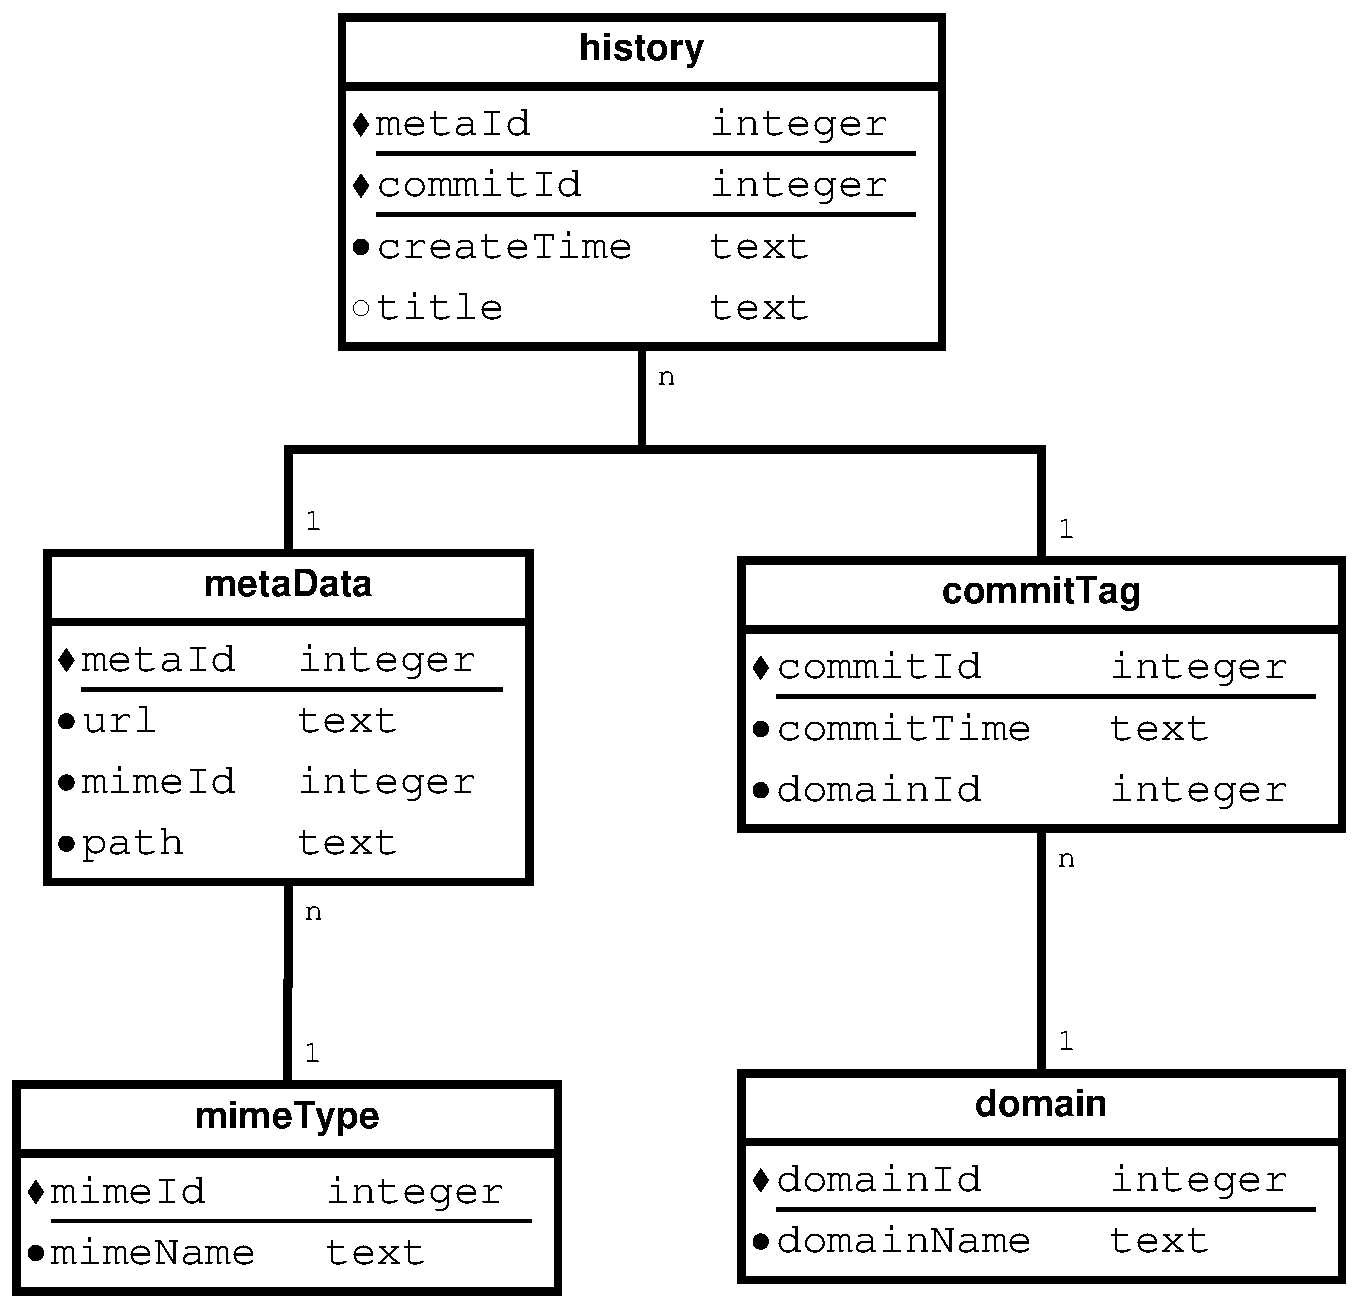
\includegraphics[width=0.6\textwidth]{design/data/db.eps}
	\caption{Datenbankdiagramm}
\end{figure}

\section{XML-Schema}
Folgendes Skripting des XML-Schemas (\ref{req:Xm:schema}) zeigt den Aufbau der XML-Datei:
\lstinputlisting[language=XML,basicstyle=\ttfamily\fontsize{8}{10}\selectfont]{../src/xml/file.xsd}
\subsection{Metadaten}
\ref{req:Xm:content:meta}
Um die Metadaten kompakter und besser lesbar zu gestalten, 
werden diese als Attribute ausgeführt. 
Dabei wird auch die 1:n-Beziehung von commitTag zu Metadaten berücksichtig:
Die commit-Daten bilden ein Unterelement von ,,meta'' und sind in diesm ebenfalls als
als Attribute enthalten.
Damit ist der commitTag auch leichter auslesbar.


Im Gegensatz zum DB-Schema erfassen die XML-Metadaten immer den gesamten Zustand innerhalb der zugehörigen Version (bzw. zu einem CommitTag), also redundant. 
\subsection{Daten}
\ref{req:Xm:content:data} \\
Das ,,data''-Element ist anfangs immer leer, kann aber durch Benutzer mittels der API-Schnittstellen 
um weitere Elemente (sog. DataElemente) erweitert.
Dabei ist auch das XSD-Schema entsprechend dem auskommentierten Template zu erweitern.
Der Name des umschließenden DataElements muss dabei einmalig sein.

Folgendes Listing zeigt ein Beispiel XML mit leerem data-Knoten:
\lstinputlisting[language=XML,basicstyle=\ttfamily\fontsize{8}{10}\selectfont]{../src/xml/example.xml}

\section{Klassen} \label{design:data:classes}
Diagramm \ref{dia:design:frontend:data:classes} zeigt die Umsetzung des Modells in Klassen.
Aufgrund der 1:n-Beziehung (siehe oben) von Metadaten und CommitTags sind die entsprechenden
Klassen auch getrennt.

Damit ist es auch möglich speicherintern CommitTags in Metadaten wiederzuverwenden.
Außerdem werden die CommitTags zur Benachrichtigung der Clients durch den Notifier benötigt
und ermöglichen ein effizienteres Auslesen aus der Datenbank.

Die TimeStamp-Klasse dient zur Vermittlung zwischen der textbasierten Speicherung von Datumswerten und der
programmierspracheninternen Darstellung z.B. java.util.Date.

Analog zu den XML-Daten enthält ein Metadatenobjekt immer den gesamten Zustand einer Datei zu einem CommitTag.

\begin{figure}[h]
	\centering
	\label{dia:design:frontend:data:classes}
	\includegraphics[width=0.7\textwidth, angle=270]{design/data/model.pdf}
	\caption{Datenbankdiagramm}
\end{figure}


\chapter{Backend}
\label{cha:backend}
% chapter backend (end)
Das Backend bezieht sich auf den in Python geschriebenen Teil, welcher öffentlich nicht sichtbar ist.

\section{Zentrale Module} 
\label{sec:zentrale_module}

\subsection{ConfigHandler}
\label{sub:confighandler}
Dieser wird zum Lesen und Setzen der Konfigurationswerte verwendet. Die Konfigurationsdatei ist in 
Xml geschreiben und hat folgenden Aufbau:

\lstinputlisting[language=XML,basicstyle=\ttfamily\fontsize{8}{10}\selectfont]{../../conf/webarchive.conf.xml}

% subsection confighandler (end)
\subsection{Commandline Interface}
\label{sub:commandline_interface}
Dieses Interface realisiert die zentralle Administrationsschnittstelle zum Webarchiv. 
Das Interface soll dabei ähnlich wie git nach dem folgenden Schema funktionieren:
\begin{verbatim}
archive [--general-options] submodule [--arguments-specific-to-submodule]
\end{verbatim}
submodule kann dabei einer der folgenden Module sein:
\begin{enumerate}
    \item init
    \item crawler
    \item javadapter 
    \item db
    \item config
\end{enumerate}

\subsection{Initialisierung} 
\label{sub:initialisierung}
Durch dieses Modul wird ein leerer Archivordner erstellt, der lediglich
ein Default-Configtemplate mit dem Pfad zum Archiv enthält, sowie einen leeren Ordner ,,content'',
in dem später die Crawldaten abgelegt werden.
Weitere Einstellung müssen händisch in der Config nachgetragen werden.
\\
Angelegt wird der Ordner über %\verbatim{archive init /pfad/zum/archive}
% subsection inititialisierung (end)

\subsection{Crawlermanager}
\label{sub:crawlermanager}
Der Crawlermanager liest eine Liste mit URLs aus einer Datei, die entweder auf der Kommandozeile oder in
der Config definiert wurde. Die URLs sind in diese Datei zeilenweise einzutragen und können durch ein \# auskommentiert werden.
Über einen ThreadPool wird dann für jede URL ein Crawljob gestartet. Die maximale Anzahl der dabei laufenden Crawljobs wird bei
der Instanzierung des ThreadPools aus der Config gelesen.
\\
Desweiteren hat der Crawlermanager nur administrative Funktionen wie dem Stoppen der laufenden Crawljobs.
% subsection crawlermanager (end)

\subsection{Crawljob}
\label{sub:crawljob}
Der Crawljob ist ein autonomer Thread der die unten aufgelisteten Submodule beeinhaltet.
Bevor die einzelnen Submodule abgearbeitet werden, wird ein temporäres Arbeitsverzeichnis angelegt.
Die Lage dieses Verzeichnisses kann in der Confug festgelegt werden.

\subsubsection{Wget}
\label{ssub:wget}
Eine Managementschicht zur Abstraktion von wget.
Dieser wird eine Domain zugeteilt welche von wget mit konfigurierbaren Parametern gecrawlt wird.
Die allgemeine Webseitenstruktur wird dabei intakt gelassen:

\begin{verbatim}
www.heise.de/
    index.html
    news/
        newsfeeds.html
        favicon.png
        ...
\end{verbatim}


\subsubsection{Cleaner}
\label{ssub:cleaner}
Der Cleaner bereingt die Verzeichnisstruktur indem er leere Ordner und Dateien löscht.
Desweiteren wird folgende Restrukturierung durchgeführt:
\begin{verbatim}
www.heise.de/ 
    index.html/
        data
    news/
        newsfeeds.html/
            data
        favicon.png/
            data
        ...
\end{verbatim}


\begin{itemize}
    \item Ordner werden intakt gelassen
    \item Für jede reguläre Datei wird ein gleichnamiges Verzeichnis angelegt
    \item Die regulären Daten werden in dieses Verzeichnis mit den Namen ,,data'' verschoben.
\end{itemize}

Außerdem werden während des Strukturierens die grundlegenden Metadatan als Liste im Speicher gesammelt.
Bevor die Datei an das Filtersystem weitergeleitet wird, wird ein ,,Titel'' abhängig vom MIME-Type ermittelt.
Pro Datei werden die konfigurierten Filter ausgeführt, welche entscheiden ob eine Datei gelöscht werden soll oder nicht.
Gibt ein Filter ,,false'' zurück, so wird der jeweilige Dateiordner samt Inhalt sowie die Metadatan gelöscht,
ohne dass weitere Filter aufgerufen werden müssen.
% subsubsection Cleaner (end)

\subsubsection{Filtersystem}
\label{ssub:filtersystem}
Das Filtersystem entscheidet aufgrund eines übergebenen Metadaten-Dictionaries ob eine Datei behalten wird. Exemplarisch wird ein HTML-Filter
implementiert. Die Filter werden jeweils in einem Subintepreter gestartet, wobei die Metadaten im Subintepreter global vorhanden sind.
% subsubsection filtersystem (end)


\subsubsection{XmlGen}
\label{ssub:xmlgen}
Hierbei werden aus der Metadatenliste Xml-Dateien zum jeweiligen Content geschrieben (data.xml). 
Beim Xml generieren werden die Metadaten mit dem aktuellen Systemdatum versehen.
% subsubsection xmlgen (end)


\subsubsection{DBGen}
\label{ssub:dbgen}
Analog zur Xmlgenerierung wird ein SQL-Statement erstellt, dass Daten aktualisiert oder neu hinzufügt.
Ist die Datenbank noch nicht vorhanden so wird sie neu erstellt.
% subsubsection dbgen (end)


\subsubsection{Rsync}
\label{ssub:rsync}
Rsync ist eine Managementschicht für das Unix Tool ,,rsync''. Rsync wird verwendet um die gecrawlten Daten sauber ins Archiv zu synchronisieren.
Hierbei wird der aktuelle gecrawlte Inhalt ins Archiv gespiegelt. 
% subsubsection rsync (end)


\subsubsection{Git}
\label{ssub:git}
Das Git Modul ist ein Wrapper für das SCM ,,git''. Es wird verwendet um das Archiv mit einer Versionierung auszustatten. Hierzu werden 
die Dateien ins Archiv per Git hinzugefügt, der Stand wird ,,commited'' und ein CommitTag generiert.
% subsubsection git (end)


% subsection crawljob (end)

\subsection{Logger}
\label{sub:logger}
Der Logger wird für das zentrale Loggen im Backend verwendet. Er implementiert die folgenden Error Level:
\begin{itemize}
    \item DEBUG
    \item CRITICAL
    \item ERROR
    \item WARNGING
    \item INFO
\end{itemize}

Folgende Funktionen werden bereitgestellt:
\begin{verbatim}
log.print(severity, *messages)
log.verbosity(SEVERITY)
\end{verbatim}
% subsection logger (end)

% subsubsection  (end)

\section{Util} 
\label{sec:util}
Das Util Modul stellt verscheidene Funktionen die von mehreren Modulen genutzt werden bereit. Erwähnenswert ist hier der ,,Lockmechanismus''
auf Dateisystemebene um Daten beim Zugriff auf gemeinsame  Ressourcen zu schützen.

% section util (end)


\section{Javadapter} 
\label{sec:javadapter}
Der ,,Javadapter'' stellt eine Schnittstelle zwischen Python und Java dar. Er ist als Daemon implementiert der über einen Socket über einen definierten Port
erreichbar ist. Interagiert werden kann mit dem Adapter über ein Textprotokoll. Der Client (in unserem Fall der Java-Server) kann bestimmte Kommandos
zeilenweise an den Server schicken, welcher dann mit ,,OK'' oder ,,ACK [Fehler]' antwortet.
\\
Folgende Kommandos sollen dabei implementiert werden:
\begin{itemize}
    \item \texttt{lock [domain]}
        Lockt eine bestimmte Domain mittels einen Lockfiles
    \item \texttt{unlock [domain]}
        Löscht ein durch \texttt{lock} erzeugtes Lockfile
\end{itemize}
% section javadapter (end)

\chapter{Frontend}

\section{Logging und Exceptionhandling}
Bei der Implementierung der Klassen wurde soweit möglich auf das Werfen von Exceptions verzichtet.
Stattdessen wird mit \lstinline{assert}-Statements gearbeitet um ungültige Eingaben, Ausgaben und Zustände schon frühzeitig während der Testphase zu erkennen. 
Diese sind dann später defaultmäßig ausgeschaltet, was die Performance verbessert.

Von Drittanbietern, bzw. der Java-Bibliothek erzeugte Exceptions werden je nach Ursache behandelt.
Interne Fehler werden geloggt und in Logfiles geschrieben. Diese befinden sich ebenfalls im installierten Archivordner.

Von Benutzern verursachte Fehler (z.B. Syntaxfehler in SQL-Klauseln) werden über einen Mechanismus
in der Server-Clientkommunikation zurückgeschickt und im Client erneut geworfen.

\section{Tests}
\subsection{ClientMockup}
	Der ClientMockup testet alle Schnittstellen zum Client, zum Backend (JavaDapter) sowie die Kommunkation übers Netzwerk.
	Dabei wird das Zusammenspiel aller Komponenten getestet.
\subsection{Unittests}
	In den Unittests wird die Funktionalität der einzelnen Klassen getestet.
	Die Tests sind packageweise in Testsuites verknüpft, welche wiederum über eine übergeordnete TestSuite aufgerufen werden können.
	Hier folgt die Erläuterung für paketweise:	
	\subsubsection{webarchive.api}
		In der API werden nur die konkreten Klassen getestet, Schnittstellen
		oder Abstraktionen werden in den konkreten Implementierungen der anderen Pakete oder im ClientMockup getestet.
		\paragraph{.model}
		Bei den Modelklassen müssen hauptsächlich Getter getestet werden.
		Außerdem werden auch illegale Eingaben in die Konstruktoren getestet,
		wobei diese nur mit asserts abgefangen werden, da Objekte später nicht
		ins System geschrieben werden können.
		\paragraph{.select}
		Die API-Selectklassen bereiten die Eingaben der Benutzer auf die
		Select-klassen im Server vor (benannte where-Parameter werden in
		eine generische Arrayform gebracht).

		Es wird deshalb getestet, ob durch Eingaben die richtige Arrayausgabeform erzeugt wird.

		Null-werte sind legal und werden als nicht vorhandene WHERE- bzw. ORDER-BY Klausel interpretiert.
		Das Erkennen von Syntaxfehlern in den Klauseln wird natürlich der Datenbank überlassen.
		\paragraph{.xml}
		Es wird die TagName-klasse getestet, welche dafür sorgt dass Xml-Tagnames mit richtigen Präfixen versehen wird. Es wird also die Erzeugung mit verschieden Eingaben und deren Ausgabe getestet.

	\subsubsection{webarchive.xml}
		Da das XML-Paket hierarchisch aufgebaut ist, sind die Tests dementsprechend gestaltet. 
		In Lowlevel-Klassen werden die Primitivfunktionen getestet, während in den Highlevel-Controllern (XmlHandler, XmlEditor) zusammengesetzte Funktionalitäten getestet werden. 

	Die Netzwerkverbindung wird dabei mit Mockupklassen umgangen. 
	Es wird auch die Konfigurierung von XmlConf mit einer Test-Configdatei geprüft.
	Desweiteren wird geprüft:
	\begin{itemize}
		\item Das Auslesen vorhandener und nicht vorhandener Datenelemente.
		\item Hinzufügen von Datenelementen, inklusive Transformation der DOM und schreiben auf die Festplatte.
		\item Die Übergabe ungültiger Werte wie null, schreibgeschützter oder bereits vorhandener DataElement-objekte, 
		\item Die Validierung: Das Anlegen von neuen Datenelementen, mit hinzugefügten gültigen Elementen in einer Test-xsd-Datei sowie das Hinzufügen invalider Elemente.
	\end{itemize}


	\subsubsection{webarchive.dbaccess}
		Die Datenbankklassen werden mithilfe einer Testdatenbank getestet, welche sich im Ordner \lstinline{test/sql} befindet.

		Bei den Typbezogenen Selects (z.B. SelectMetaDataTest) wird getestet, 
		ob das Mapping zwischen relationeller DB und Objekten funktioniert.
		Außerdem werden erwartete Testwerte aus der Datenbank abgeprüft.
		
		Die abstrakte Klasse SelectJoin wird dahingehend getestet, 
		dass vorbereite SELECT-Statements anhand der übergebenen Parameter richtig zusammengesetzt werden.
		Diese SELECTs werden dann anschließend mit verschiedenen Pseudo-WHERE- und ORDER-BY-Klauseln gefüllt
		und die Syntax geprüft.
		Desweiteren sollen SQL-injections durch interne Abfragen verhindert werden.

		Die Klasse SqlHandler, welche als Fassadenschnittstelle nach aussen dient, wird daraufhin
		geprüft, dass übergeben Select-objekte (aus dem api-package) den richtigen Ausführungsselects zugeordnet werden. Das Ergebnis kann wiederum anhand erwartbar Rückgabewerte geprüft werden.

\end{document}

